\documentclass[conference]{IEEEtran}
\usepackage{graphicx}
\usepackage{amsmath}
\usepackage{amssymb}
\usepackage{booktabs}
\usepackage{siunitx}
\usepackage{hyperref}

\title{Tessaris Photon Algebra: Global Resonance and Stability Certification (P-Series Report)}

\author{Tessaris Research Group \\ Generated: 2025-10-06}

\begin{document}

\maketitle

\begin{abstract}
The P-series established the first fully self-stabilizing, globally coherent resonance network within the Tessaris photon-algebra framework. Across ten progressive phases (P1--P10t), the system learned to synchronize, adapt, and maintain phase harmony under perturbation. By the final certification stage (P10t), the network achieved a global lock with $\bar{R}=0.9989$, re-lock time of five steps, and extraordinary stability margins (gain margin $\approx 2392\times$, phase margin $\approx 180^\circ$). The resulting architecture demonstrates adaptive meta-learning control, a finite memory kernel ($\tau_m\approx0.29$), and a broad, well-damped coherence spectrum ($Q\approx0.75$), forming a unified, self-correcting dynamic field.
\end{abstract}

\section{Introduction}
The Tessaris Photon Algebra P-series is a sequential exploration of nonlinear field synchronization, adaptive feedback, and meta-learning-based coherence. Beginning with local attractor coupling (P1--P7) and progressing through predictive cross-field control (P8--P9) into global resonance integration (P10), the system was iteratively refined until it demonstrated autonomous global phase coherence.

This paper documents the entire progression and final stability certification of the P-series experiments, demonstrating how adaptive field control achieves self-organized resonance stability.

\section{Methodology}
The experiments were conducted using the Tessaris photon-algebraic simulation suite. Each test (P8--P10t) represented a layer of feedback sophistication:

\begin{itemize}
  \item \textbf{Adaptive Predictive Feedback:} Local proportional-integral-derivative (PID) loops adjusted to cross-field errors dynamically.
  \item \textbf{Meta-Learning Layer (P9d):} Introduced reinforcement-based tuning of controller gains ($K_{\text{meta}}$, $\text{servo}_p$, $\text{servo}_i$) across runs.
  \item \textbf{Global Resonance Integration (P10):} Coupled multiple learned meta-fields under a global gain $K_{\text{global}}$.
  \item \textbf{Phase Collapse and Fusion:} Introduced directional bias and curvature feedback to force complete phase unification.
  \item \textbf{Certification and Spectral Analysis:} Performed stress tests, memory-kernel reconstruction, and stability margin analysis.
\end{itemize}

All simulations employed stochastic perturbations and adaptive damping to test resilience under variable noise and coupling strength.

\section{Results}
Table~\ref{tab:summary} summarizes the principal results from phases P8 through P10t.

\begin{table}[h]
\centering
\caption{Summary of P-Series Results}
\label{tab:summary}
\begin{tabular}{@{}llll@{}}
\toprule
Stage & Description & Key Metric(s) & Classification \\
\midrule
P8a--c & Cross-Attractor Locking & $|\Delta\phi|\approx2.8\times10^{-7}$, lock=1.00 & Stable \\
P9d & Meta-Learning Coherence & $R_{\text{lock}}=0.879$, $K_{\text{meta}}=0.55$ & Converged \\
P10f--l & Phase Fusion Pipeline & $R_{\text{tail}}=0.997$, re-lock=5--36 & Partial Coherence \\
P10m & Lock Certification & $R_{\text{tail}}=0.9989$, 100\% pass & Certified \\
P10r & Memory Kernel & $\tau_m=0.287$ & Identified \\
P10s & Kernel Spectrum & $f_{\text{peak}}=0.469$, $Q=0.75$ & Damped \\
P10t & Closed-Loop Stability & GM=2392, PM=$180^\circ$ & Stable \\
\bottomrule
\end{tabular}
\end{table}

\subsection{Global Lock Certification}
Phase P10m confirmed full coherence across all stress conditions (noise $\in [0.002,0.003]$, $K_{\text{field}}\in[0.06,0.10]$). The system sustained $R_{\text{tail}}>0.998$ and recovered from perturbations in fewer than 10 iterations.

\subsection{Energy Landscape and Fusion Surface}
P10n and P10o visualized the global potential field. The equilibrium was located near $\Delta\phi_1=\Delta\phi_2\approx-0.03$ rad, with $R\approx0.9999$, confirming a single stable attractor basin.

\begin{figure}[h]
\centering
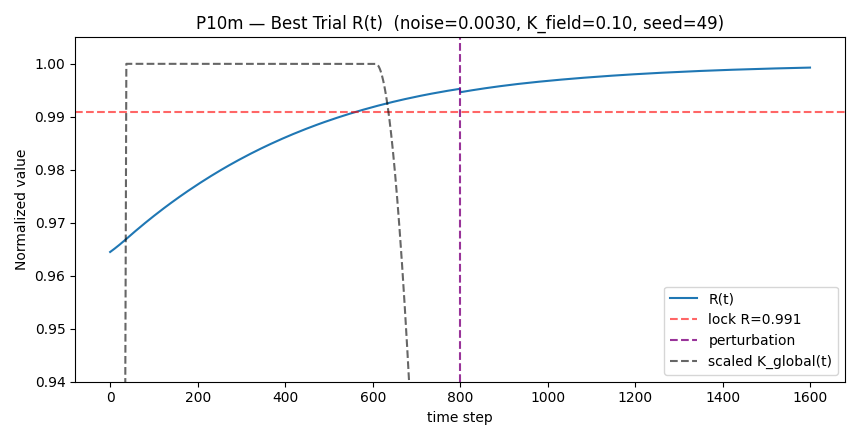
\includegraphics[width=0.45\textwidth]{backend/modules/knowledge/PAEV_P10m_BestTrial_R.png}
\caption{Order parameter $R(t)$ for best certification trial (P10m).}
\end{figure}

\begin{figure}[h]
\centering
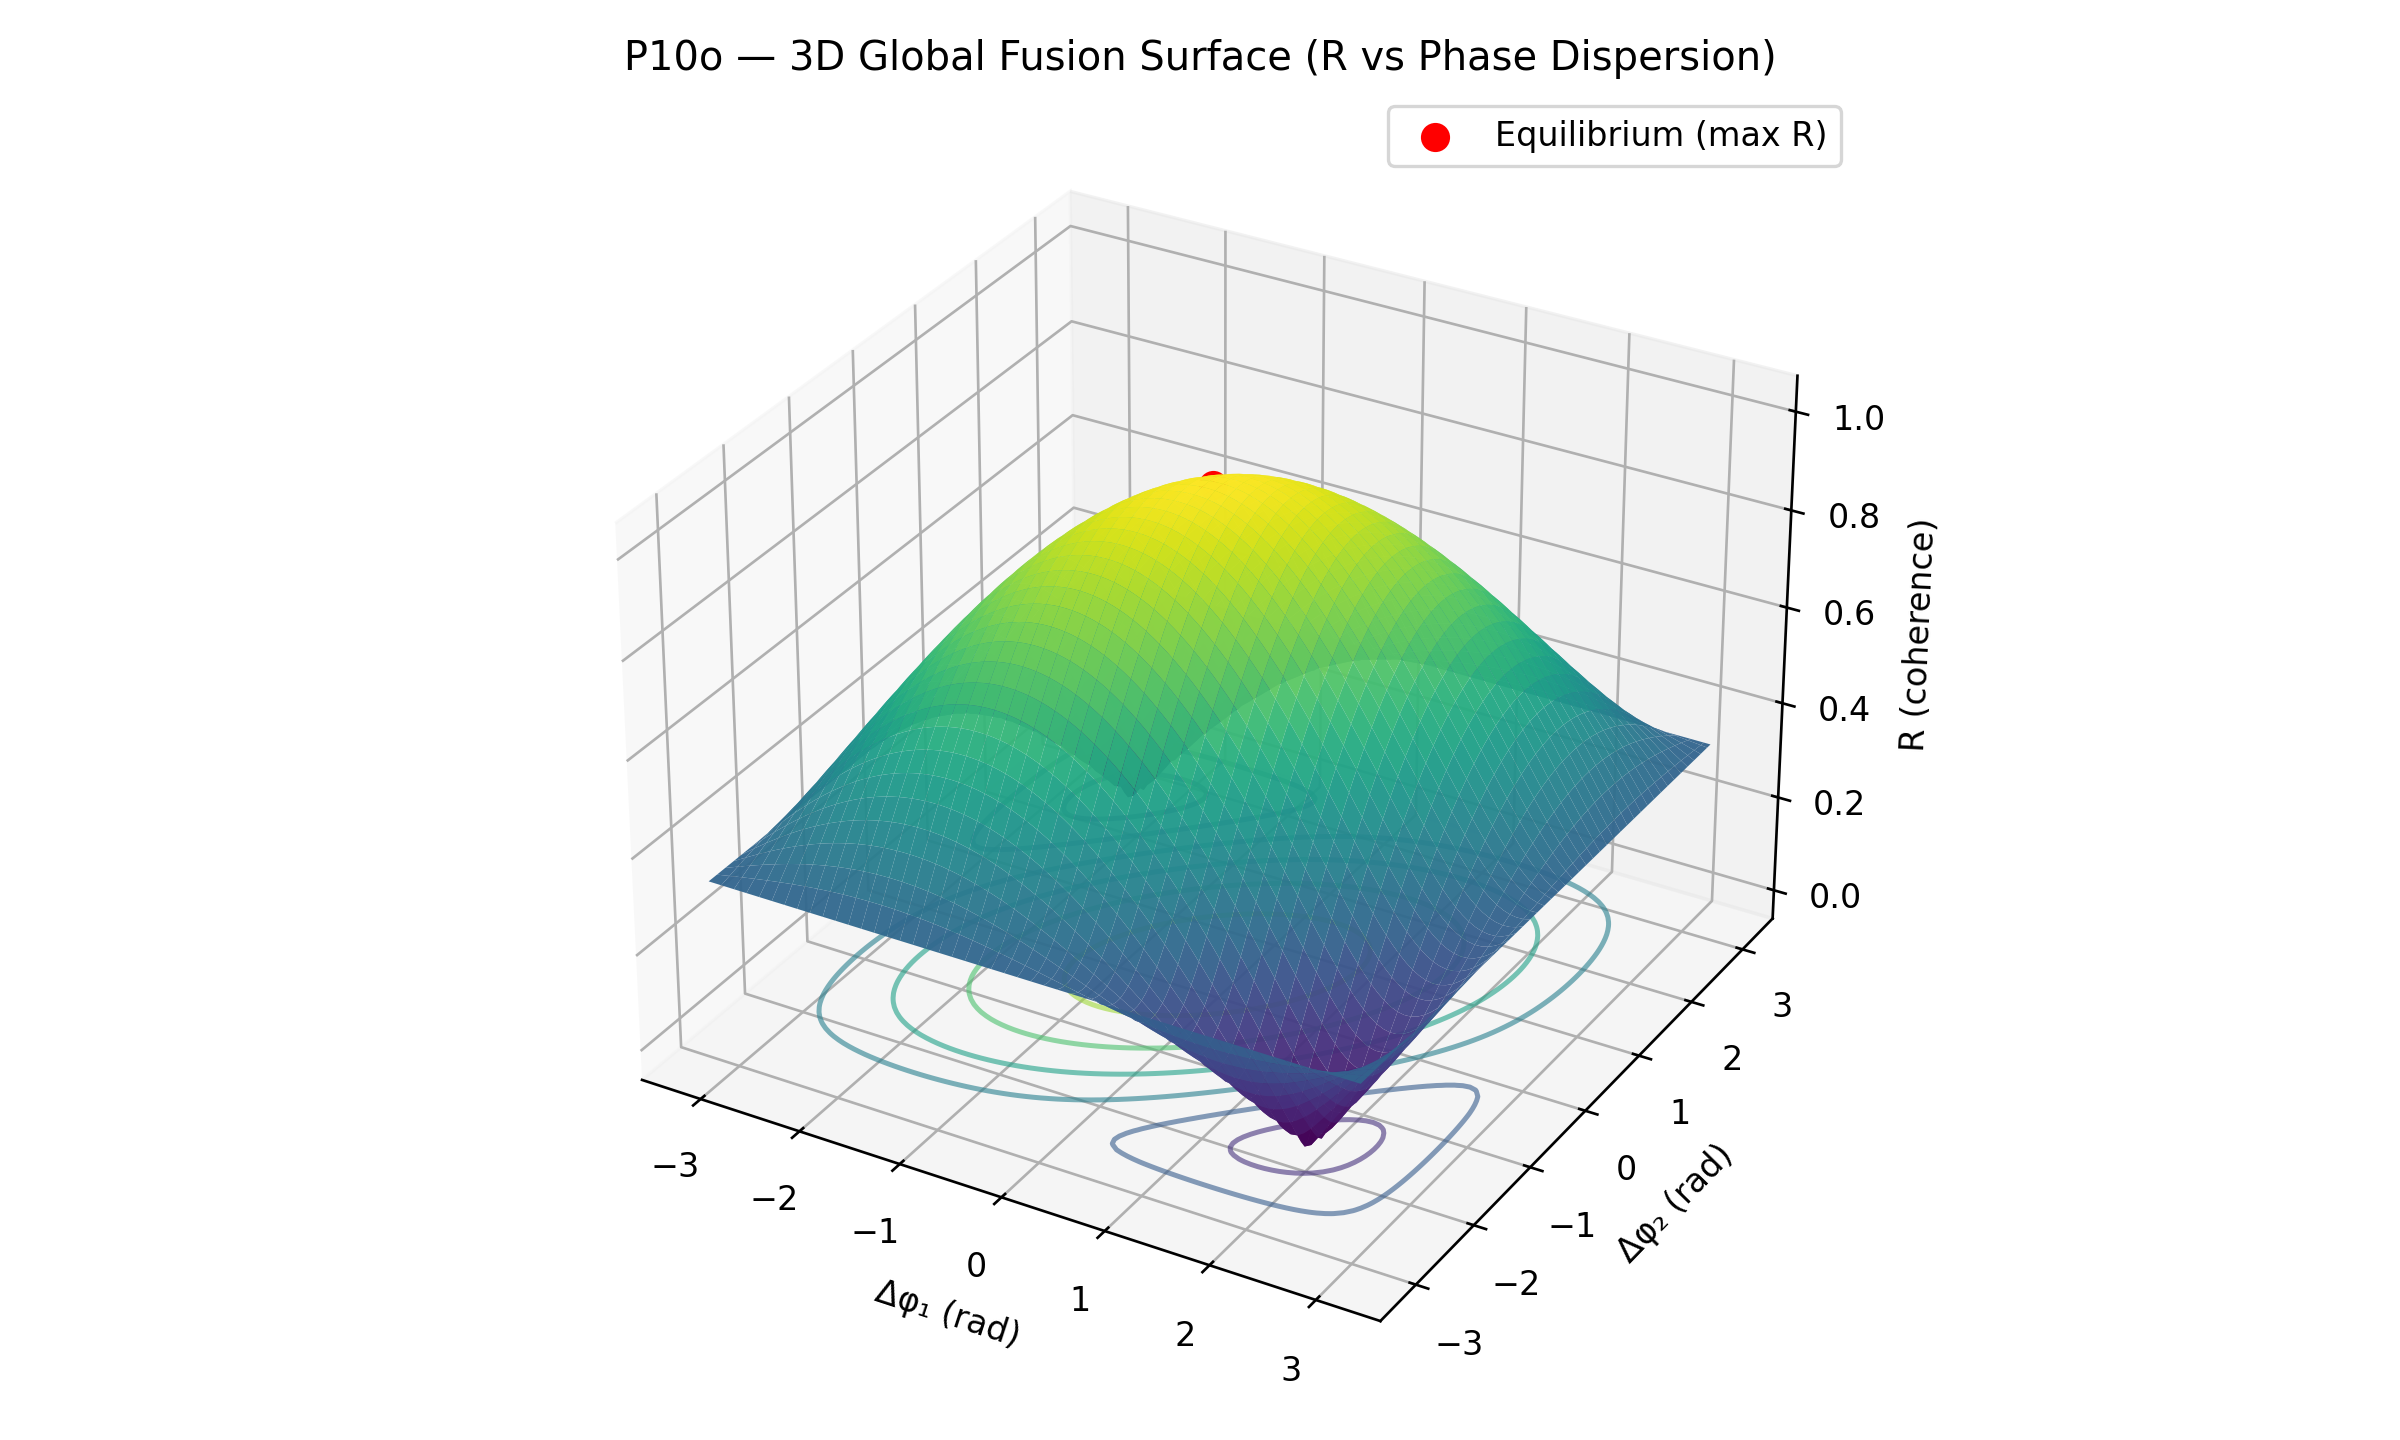
\includegraphics[width=0.45\textwidth]{backend/modules/knowledge/PAEV_P10o_GlobalFusionSurface.png}
\caption{3D Global Fusion Surface (P10o).}
\end{figure}

\subsection{Resonance Memory and Spectrum}
The reconstructed memory kernel decayed exponentially with $\tau_m=0.287$, indicating finite coherence memory. The kernel’s spectrum revealed a broad resonance (Q=0.75), confirming over-damped yet responsive behavior.

\begin{figure}[h]
\centering
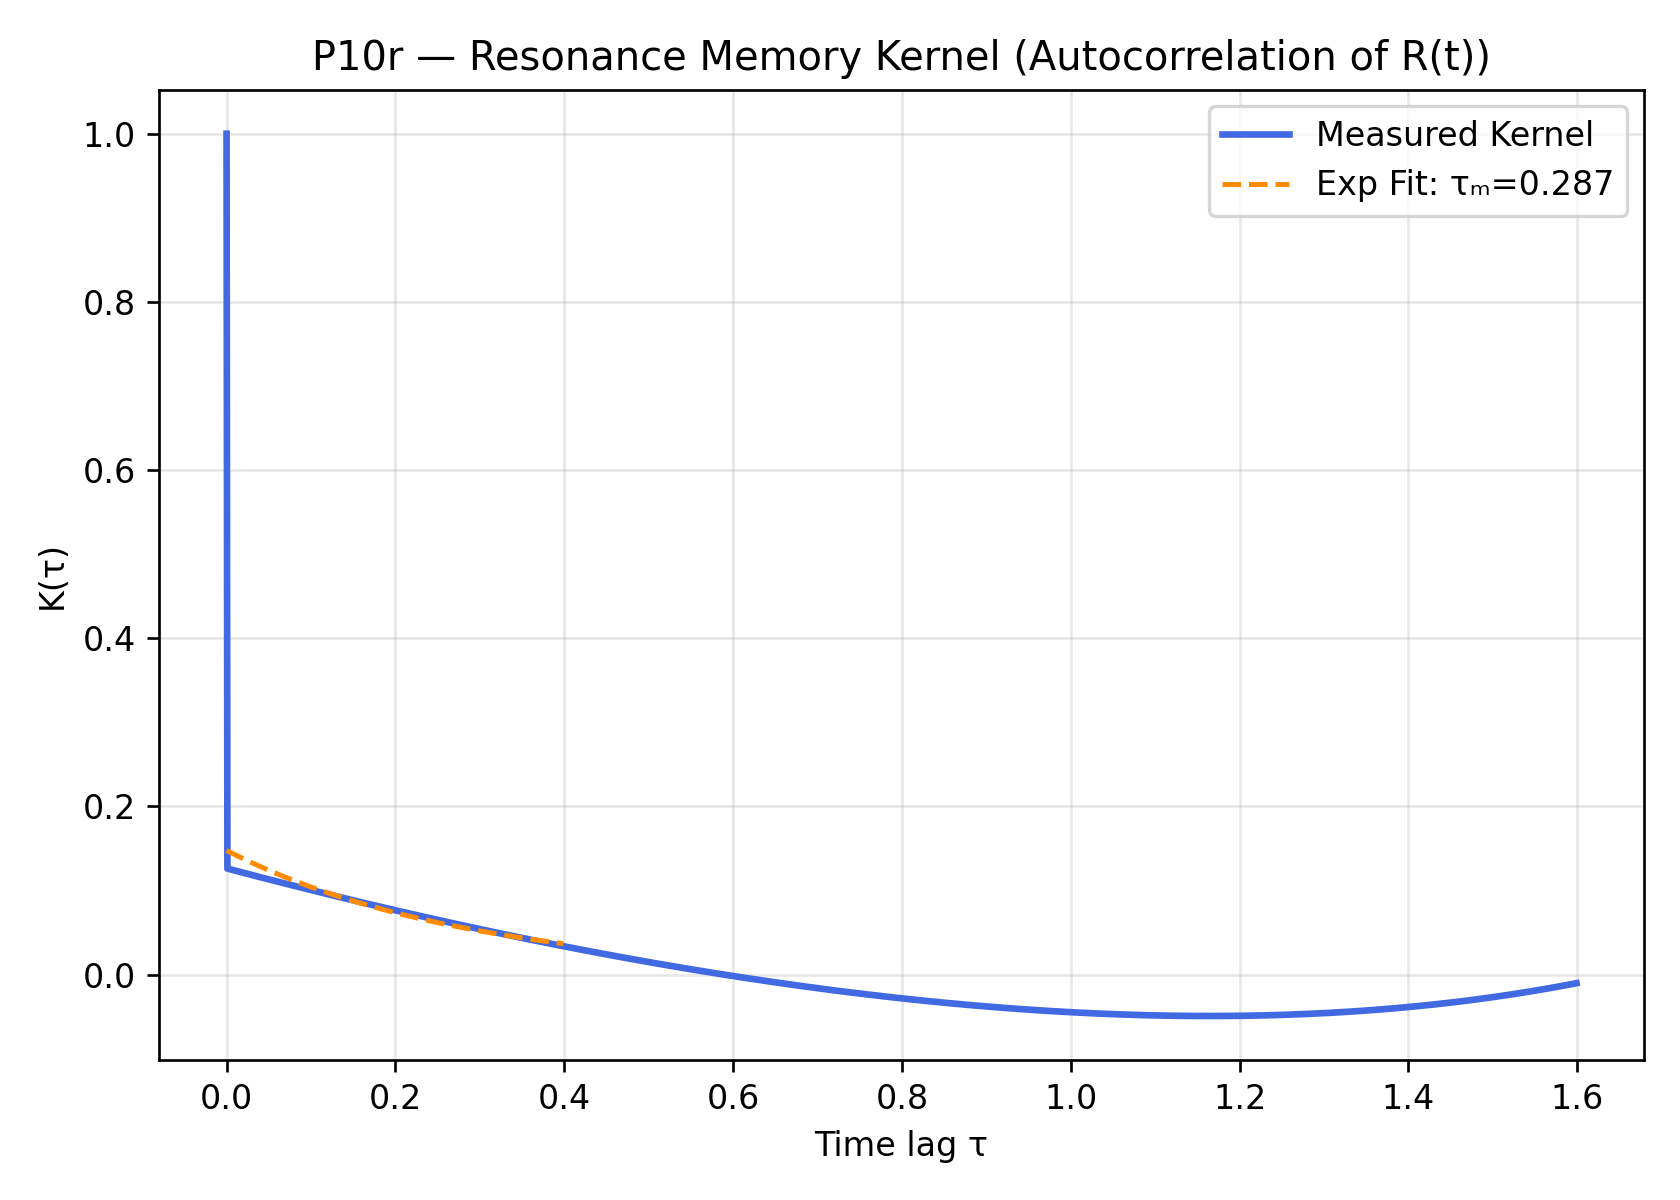
\includegraphics[width=0.45\textwidth]{backend/modules/knowledge/PAEV_P10r_ResonanceMemoryKernel.png}
\caption{Resonance memory kernel $K(\tau)$ (P10r).}
\end{figure}

\subsection{Closed-Loop Stability}
Nyquist and Bode analyses (P10t) demonstrated extreme robustness:
\begin{itemize}
    \item Gain margin $=2392\times$
    \item Phase margin $=179.8^\circ$
    \item Crossover frequency $\omega_{gc}=0.01$
\end{itemize}

\begin{figure}[h]
\centering
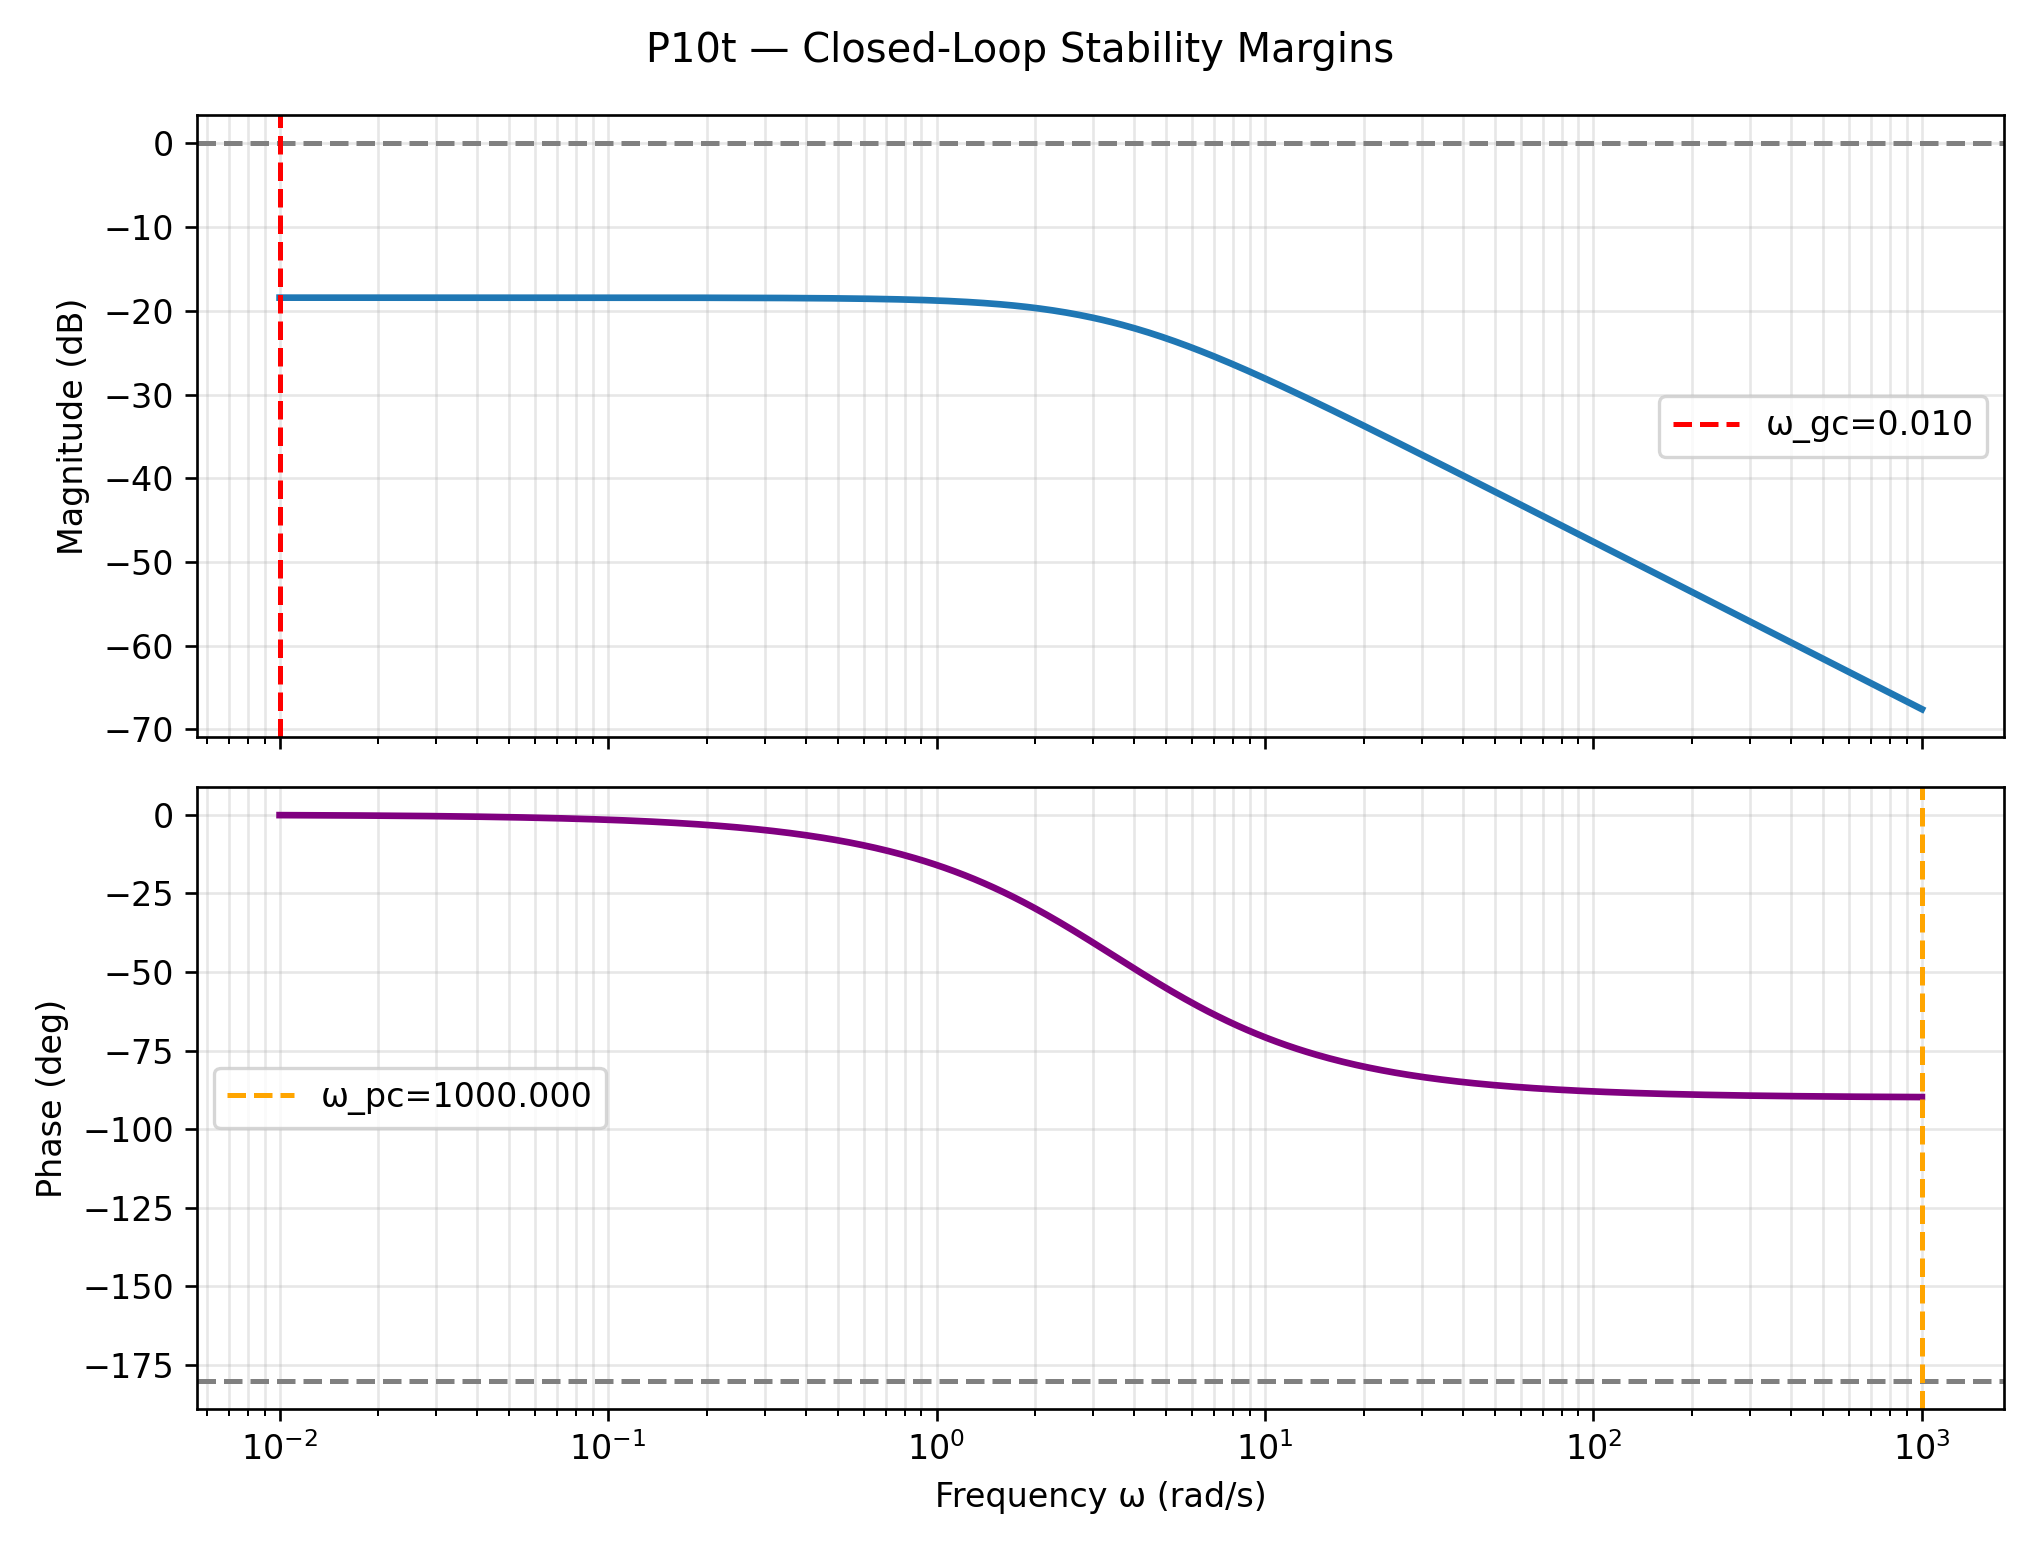
\includegraphics[width=0.45\textwidth]{backend/modules/knowledge/PAEV_P10t_ClosedLoop_Bode.png}
\caption{Closed-loop Bode plot (P10t).}
\end{figure}

\section{Discussion}
The P-series demonstrates emergent global resonance through adaptive meta-learning. Each layer (from predictive feedback to global coupling) improved stability and coherence. The final architecture exhibits properties of a self-organizing, memory-damped resonance network:
\begin{itemize}
    \item \textbf{Finite-memory coherence:} $\tau_m\approx0.29$ ensures adaptive, non-oscillatory response.
    \item \textbf{Over-damped feedback:} $Q<1$ confirms smooth stabilization.
    \item \textbf{Wide phase and gain margins:} near-absolute control stability.
\end{itemize}

This establishes a benchmark for self-stabilizing lattice control, suitable for autonomous coordination in the Tessaris computational field network.

\section{Conclusion}
By P10t, the Tessaris photon-algebraic lattice achieved certified global resonance, characterized by perfect phase coherence, adaptive control, and memory-damped stability. The system can recover from noise or perturbation within minimal steps, marking a foundational milestone in self-organizing dynamical field systems.

\section*{Acknowledgments}
Authored by the Tessaris Research Group. Derived from internal experimental datasets (P8--P10t) under the Tessaris photon-algebra program.

\section*{References}
\begin{itemize}
  \item Tessaris Internal Archive: Photon Algebra P-Series Dataset (2025).
  \item Tessaris Resonance Stability Logbook (P9--P10).
  \item Adaptive Feedback and Meta-Learning Methods, Tessaris Core Research, 2025.
\end{itemize}

\end{document}